\section{Introduction}
\label{sec:intro}

Page Load Time (PLT) of a website is a key performance metric that
significantly impacts user-experience, as pointed out by many recent studies
from both academia and industry~\cite{bhatti2000integrating, bouch2000quality}.
User-experience in web browsing is directly correlated to companies' revenues:
Amazon shows that reducing 100ms in PLT results in 1 percent revenue increase
and Shopzilla reports that improving PLT from 6 to 1.2 seconds increased the
revenue by 12 percent~\cite{url3}. 

There have been many prior works in improving webpage's PLT of mobile devices,
ranging from offloading computation and network tasks to
proxies~\cite{netravali2015mahimahi, sivakumar2014parcel, wang2014speedy} to
re-prioritising requests at client side by letting the client itself discover
all resources on a page~\cite{butkiewicz2015klotski, netravali2016polaris}.  It
is worthwhile to note that existing works attempt to surrogate web-tasks of
mobile devices from resource-rich server
environment~\cite{ruamviboonsuk2017vroom}.
 
The end-to-end PLT for many webpages is far from the ideal: an order
of tens of seconds on mobile devices~\cite{wang2013demystifying} and
order of seconds on stationary desktops.  Many existing solutions
often require server-side modification, which strongly discourages
content providers to use new solution. 
% Joseph: why doing at server-side is bad?
Whereas a client side solution would be agnostic of the content
provider/server that is being used to render the web pages and
optimize page load times for all web pages alike. 
Most of the existing work on client side talks about efficient ways to
optimise web cache~\cite{wang2014much}.  
Prior work shows how computation latency is the driving factor behind
large web page load time, as compared to network
latency~\cite{vesuna2016caching}.

In this work, we propose PLT optimization technique that caches output
from previous code execution of a webpage (e.g., Javascript, inline
HTML, css) on mobile devices to reduce user-perceiving PLT in exchange
of prevalent mass-storage.
Prior techniques have gone as far as caching the compiled code either
on the client side or on the server side to save on the compilation
time when the web content remains unchanged~\cite{wang2014much}. We
take this a step further, and cache the output of the execution of all
the code on a web page. ( Note that I use the word code, to
distinguish it from other components of a webpage which include layout
and data). Recent work has shown that most of the webpages remain
unchanged over a large period of time. For content-rich pages, the
amount of updates vary across Web pages. In the best (worst) case,
20\% (75\%) of the HTML page is changed over a month. Most changes are
made to data (e.g., links to images, titles) while little is made to
layout and code~\cite{wang2014much}.  This implies that most of the
code output could be reused, essentially eliminating code execution
time from the critical path of a web page load. This would bring down
the entire page load time to the time taken in rendering/painting the
layout. 
Caching the computation as a technique to optimize the execution time has
already been explored at a data center level~\cite{gunda2010nectar} and it has
shown tremendous improvement with more than 35\% job benefiting from caching.
We are trying to apply a similar technique however on the client side at a
browser level. 

\begin{figure*}[!bth]
\begin{subfigure}[h]{0.5\textwidth}
\centering
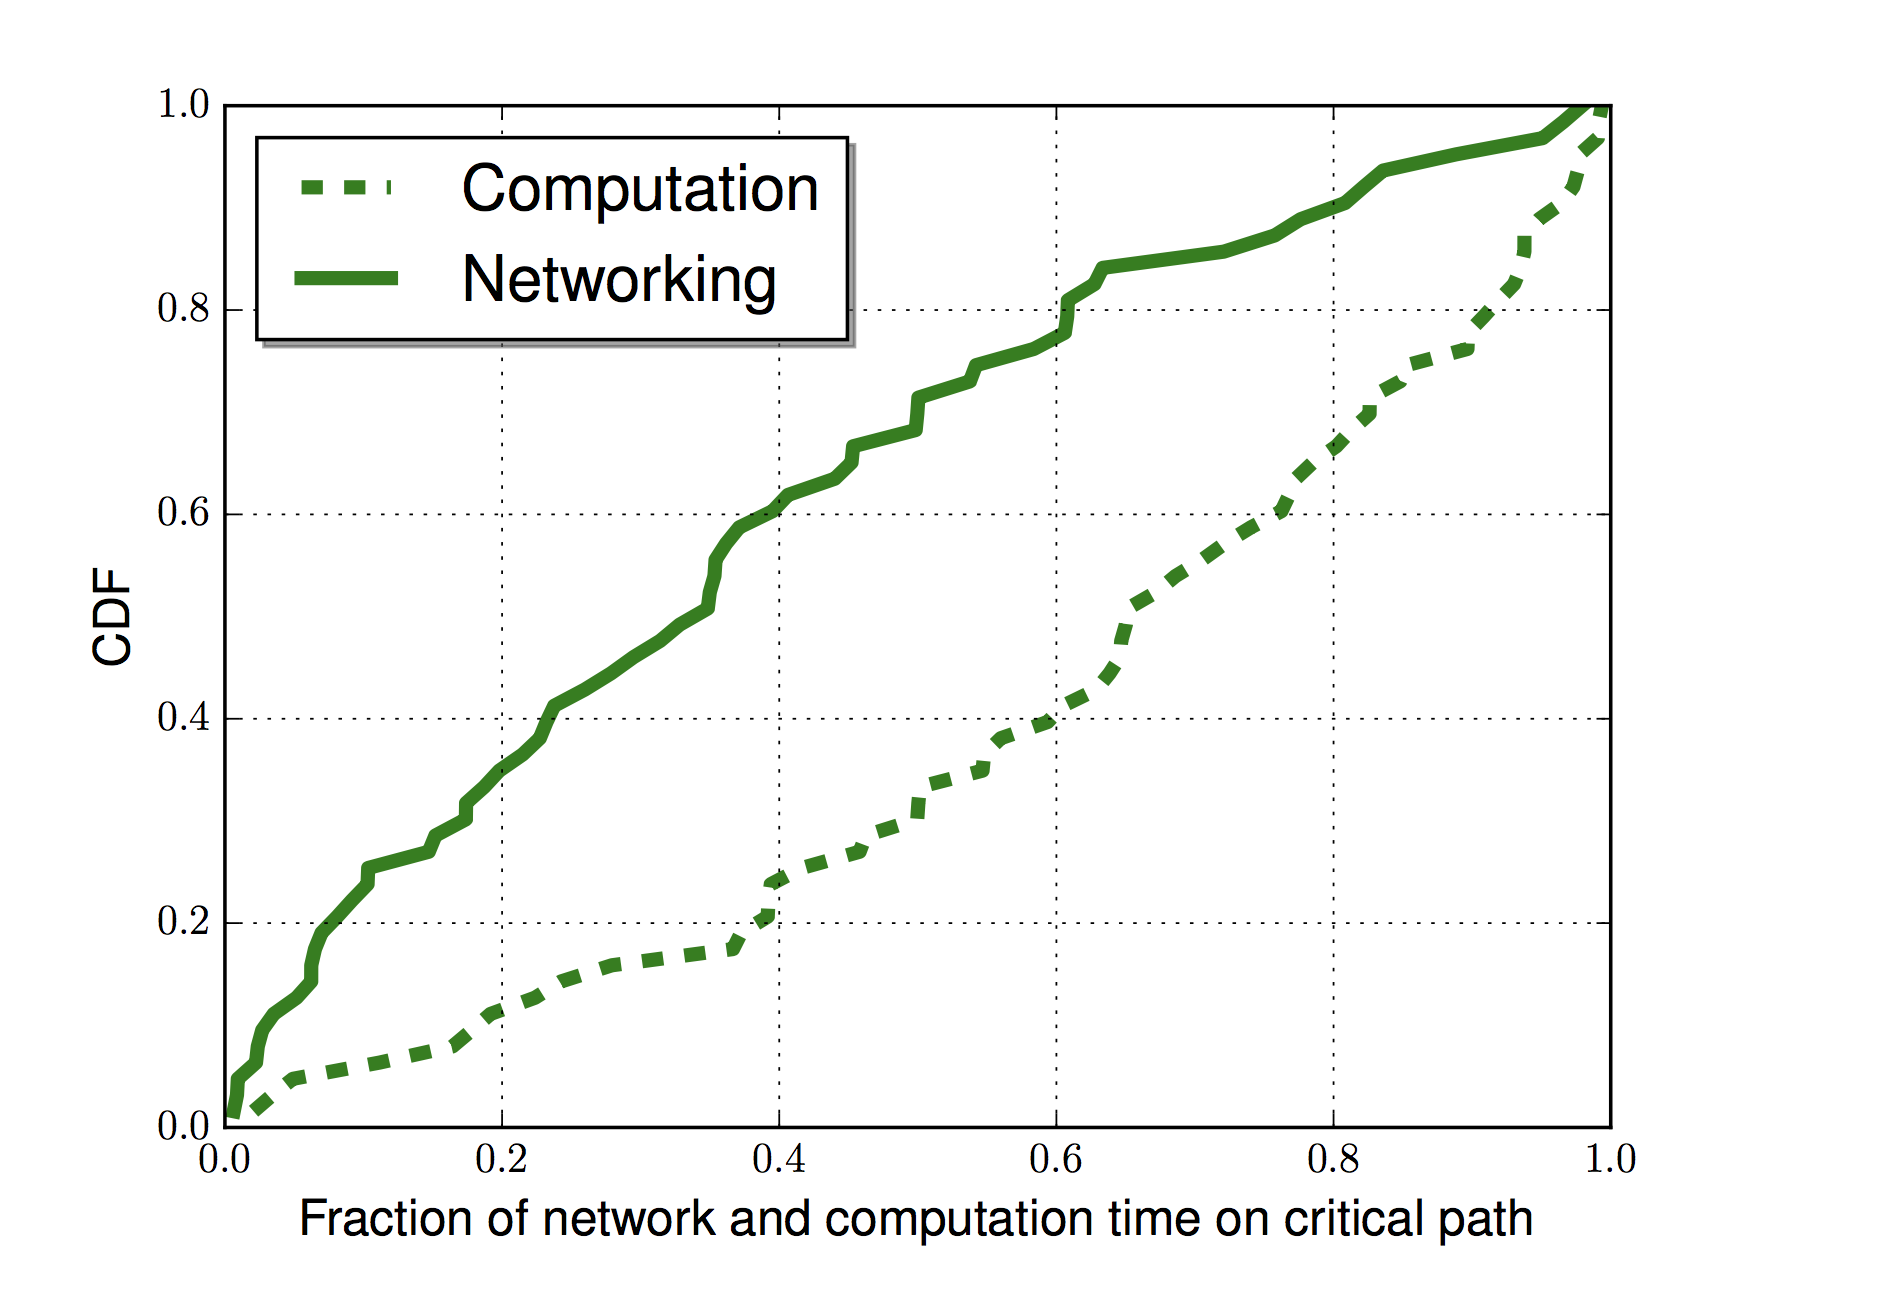
\includegraphics[width=\linewidth]{figs/comp_net.png}
\caption{Runtime information on mobile devices}
\label{fig:mobile-runtime}
\end{subfigure}
\begin{subfigure}[h]{0.5\textwidth}
\centering
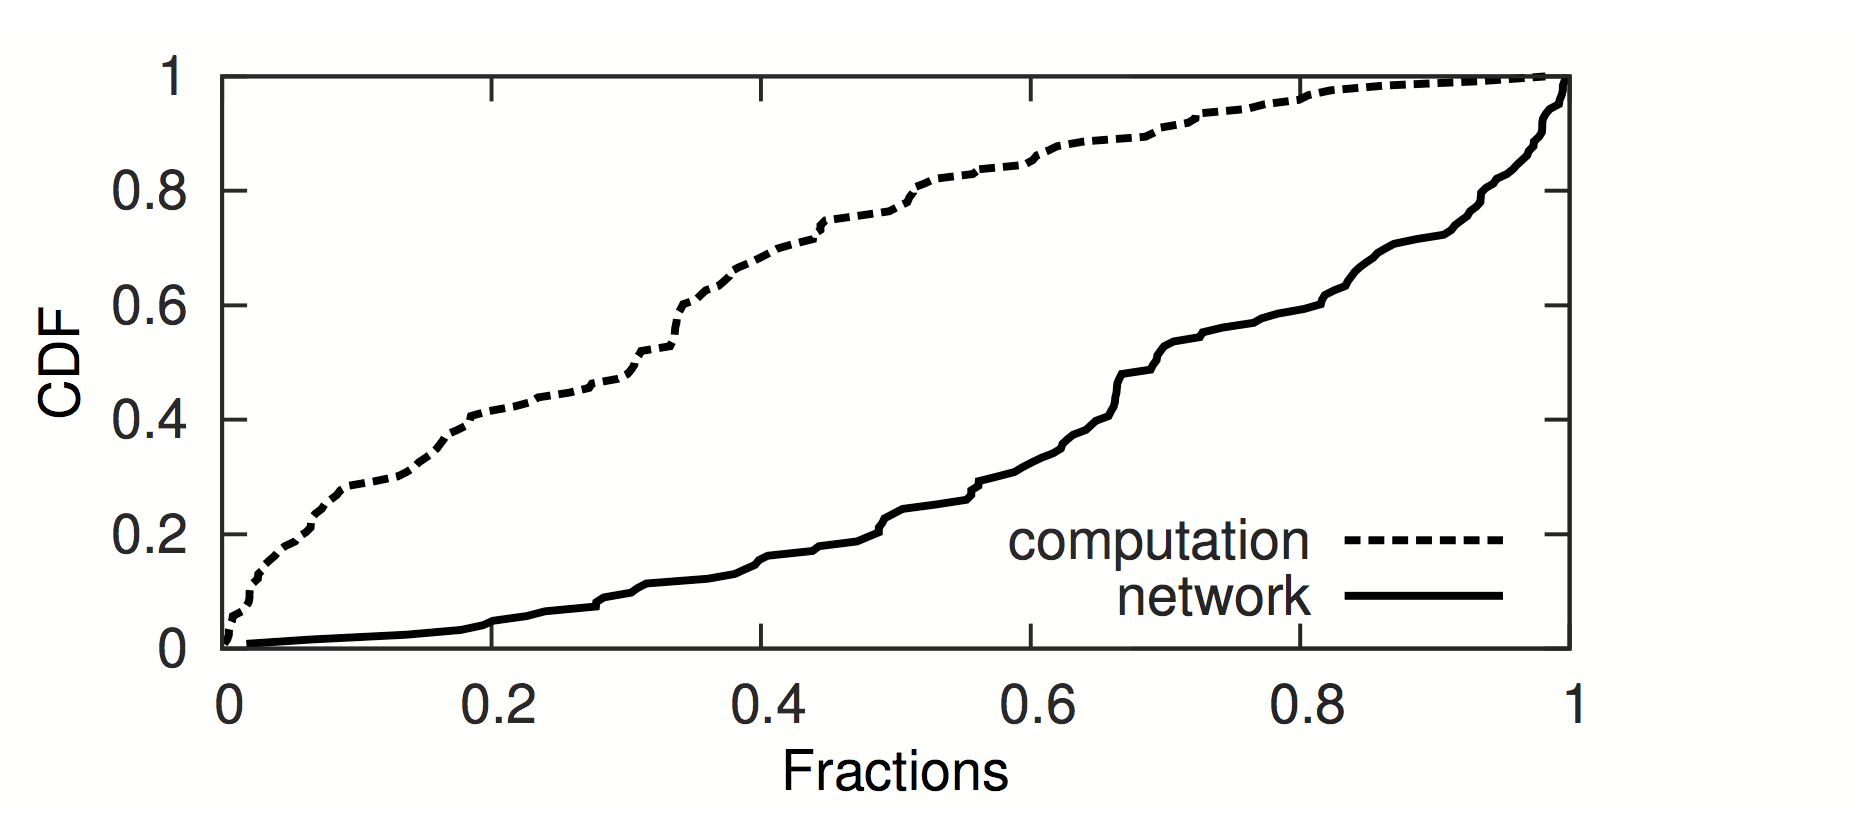
\includegraphics[width=\linewidth]{figs/comp_net_desk.png}
\caption{Runtime information on desktops}
\label{fig:mobile-runtime}
\end{subfigure}
\caption{{\color{red}Figure 1 captioon placeholder}}
\end{figure*}

